\documentclass[openany]{book}
\usepackage[utf8]{inputenc}
\usepackage{graphicx}
\usepackage[a4paper, total={6in, 8in}]{geometry}
\renewcommand{\baselinestretch}{1.4}

\title{AMME4111 Thesis A Progress Report}
\author{Joseph Daniel}
\date{October 2019}

\begin{document}

\maketitle

\tableofcontents

\chapter{Introduction}
Humans have a remarkable ability to perceive visual stimuli emanating from the world around them. Not only do we identify different objects, scene depth, movement, and colour with ease, but we often draw meaning and even enjoyment from the combination of light rays bouncing around space and arriving at our eyes. We are able to automatically compensate for differences in lighting and viewing angle, and we can extract complex information such as emotion from what we process visually. To word it concisely, the human visual perception system is one of the most versatile and robust image processing machines that we know of. Most man-made machines on the other hand are much more easily decomposed into a set of deterministic modules that require explicit, well defined instruction sets. Often, when given an image, there is no straightforward function that directly maps from pixel intensities to the semantic meaning of that image. As researchers tackling problems in computer vision, we are usually interested in developing the algorithms that can help machines not only sense the world, but perceive it in a way that is useful.The objective of this thesis project is to develop a pipeline that simultaneously learns to perform two tasks. The first is visual odometry - the act of estimating camera motion from a sequence of images. The growth of autonomous robotics has meant that there is an every-growing need for accurate navigation and localisation when satellite positioning is unavailable or wheel encoder odometry is unreliable. An autonomous unmanned aerial vehicle navigating an unknown indoor environment is one example where visual odometry is a valuable feedback signal that can be used to precisely control the UAV's position. The second is depth estimation, that is, discerning the distance of objects in a scene from the imaging device. The ability to perform depth estimation from visual cues is desirable in applications such as autonomous vehicles where navigating new environments whilst avoiding collisions is a basic requirement. Being able to draw depth information from a camera sensor will help to enable these capabilities, especially in applications where methods such as Lidar or RGBD sensors are prohibitive - small quad-copters and internal medical imaging devices are examples where this might be the case.


Humans are exceptionally well adapted to these tasks - our two eyes allow us to process the 3D geometry of the scene, while our learned experiences are often able to fill in the gaps where geometric information is insufficient or unavailable. Unfortunately, image processing algorithms are not equipped with this same kind of human intuition, and so the deceptively complex task of estimating the 3D structure of a scene from a sequence of images continues to attract attention from the computer vision community. 


The price of camera components is decreasing while image quality continues to improve, not only making cameras an attractive perception module for autonomous robotics, but also spurring the popularity of multiple-view imaging. Embracing this idea, this thesis project seeks to develop a pipeline that performs these tasks by taking advantage of the rich geometric information exposed when using multiple views. Thus, this thesis project adopts the vocabulary and the concepts from the area of light field imaging. The light field describes the intensities and directions of each light ray in space, providing a convenient way of thinking about multi-view geometry which is embraced throughout this thesis.


Another core objective of this thesis is to develop a pipeline that relies principally on unsupervised machine learning models to perform the two tasks side-by-side. This approach is chosen with the intention that a data-driven model can build a robustness to scenarios that are difficult to design for using hand crafted solutions.  Furthermore, this pipeline will benefit from being self-supervised - unlike data-driven models that require direct supervision from a human to improve their performance (classifying images of cats and dogs is a common example), this pipeline has no intermediary requirements between the data collection and training routines. Not only does this mean that the expensive process of hand-labelling data is unnecessary for this pipeline to function, but the model will be able to continue training, benefiting from new data that it receives \textit{whilst operational in the field}. An adaptive perception module that learns to operate effectively in new environments is a desirable capability in robotics, especially when considering that effects such as thermal expansion, vibration and shocks can frequently render our equipment calibrations meaningless. 


In this progress report we will first establish the conceptual groundwork that this thesis builds upon with a discussion surrounding the seminal texts that have shaped the state-of-the-art literature in visual odometry and depth estimation. In understanding those texts, we demonstrate that existing methods have yielded excellent results, whilst identifying that there is a substantial potential for improvement on state-of-the-art results using multi-view imaging devices. 


\chapter{Literature Survey}

\section{The Light Field and Multiple View Geometry}

Light field imaging has emerged as a powerful tool in computer vision for robotics, offering a rich higher-dimensional representation than what can be captured by conventional optics. The underlying principle used to describe the light field is the plenoptic function, a 7-dimensional mapping that assigns radiance values to the light rays at every position in space, in every orientation, at all wavelengths, throughout all of time \cite{ihrke2016lfprinciples}. \cite{adelson1991plenoptic} shows that this can be formally expressed as $L(x,y,z,\theta, \phi, \lambda, t)$, and measured in $W/m^2/sr/nm/s$. 
With the addition of practical constraints however, the plenoptic function can be expressed more concisely as a parameterisation of 4 variables. 

Pixels on camera sensors integrate the number of photons arriving at them over a finite period of time removing the temporal dimension, and each colour channel can be thought of as a monochromatic sampling of the light field, removing the spectral dimension. Additionally, and importantly, is the constraint that the radiance of light rays propagating through a vacuum do not change if samples are restricted to the convex hull of the scene, thus reducing the overall dimensionality of the plenoptic function by one parameter \cite{levoy1996lfrendering}. To illustrate this, one could think of the light rays leaving the inside of a bowl sat upright on a table. Many of those rays may only travel a small distance before being blocked by the inside of the bowl itself, meaning those rays will never be registered by any practical measurement device. As shown in figure \ref{convexhull} if we consider only the convex hull of the bowl however, we are required only to represent the value of the plenoptic function on the encapsulating surface of the object \cite{gortler1996lumigraph}.

\begin{figure}[htbp]
    \centering
    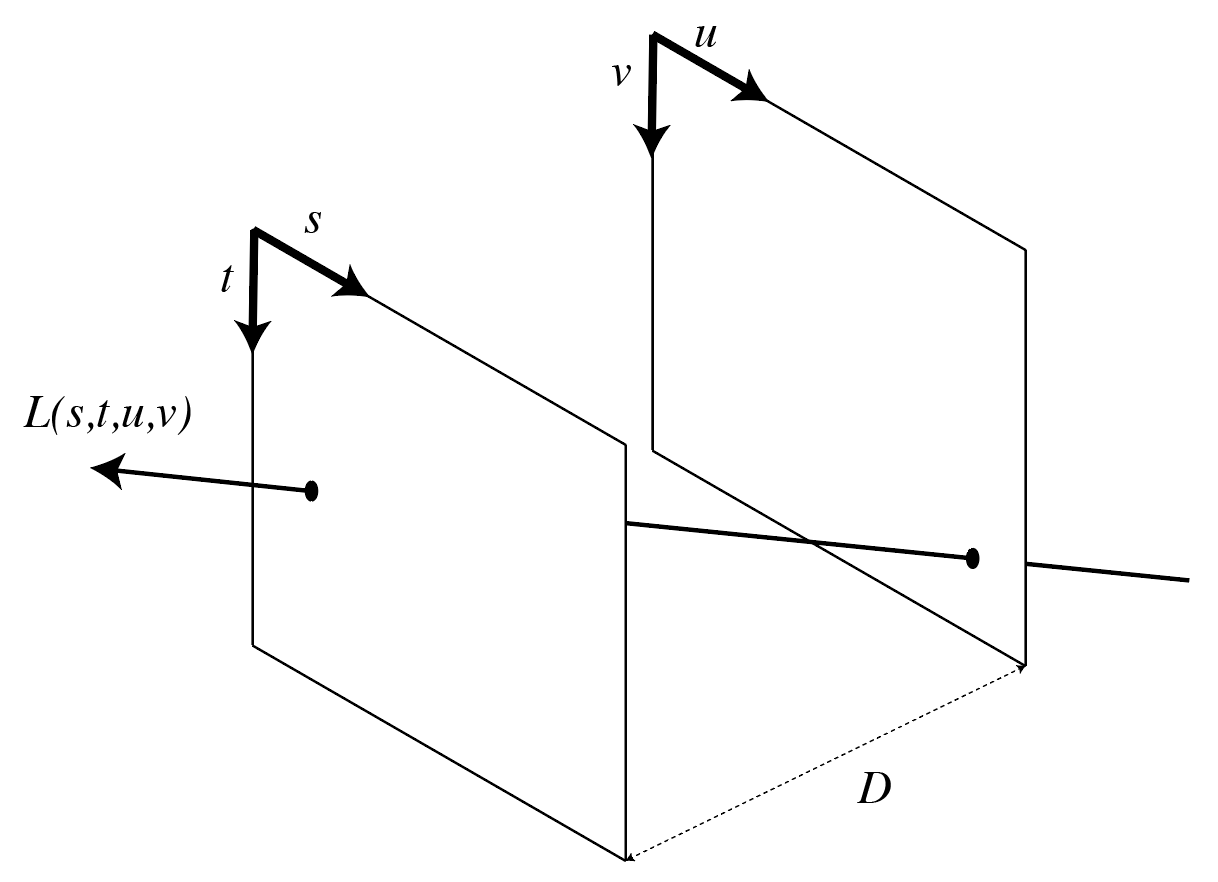
\includegraphics[width=2.5in]{images/2pp.png}
    
\includegraphics[width=0.3in]{images/blank.png}
    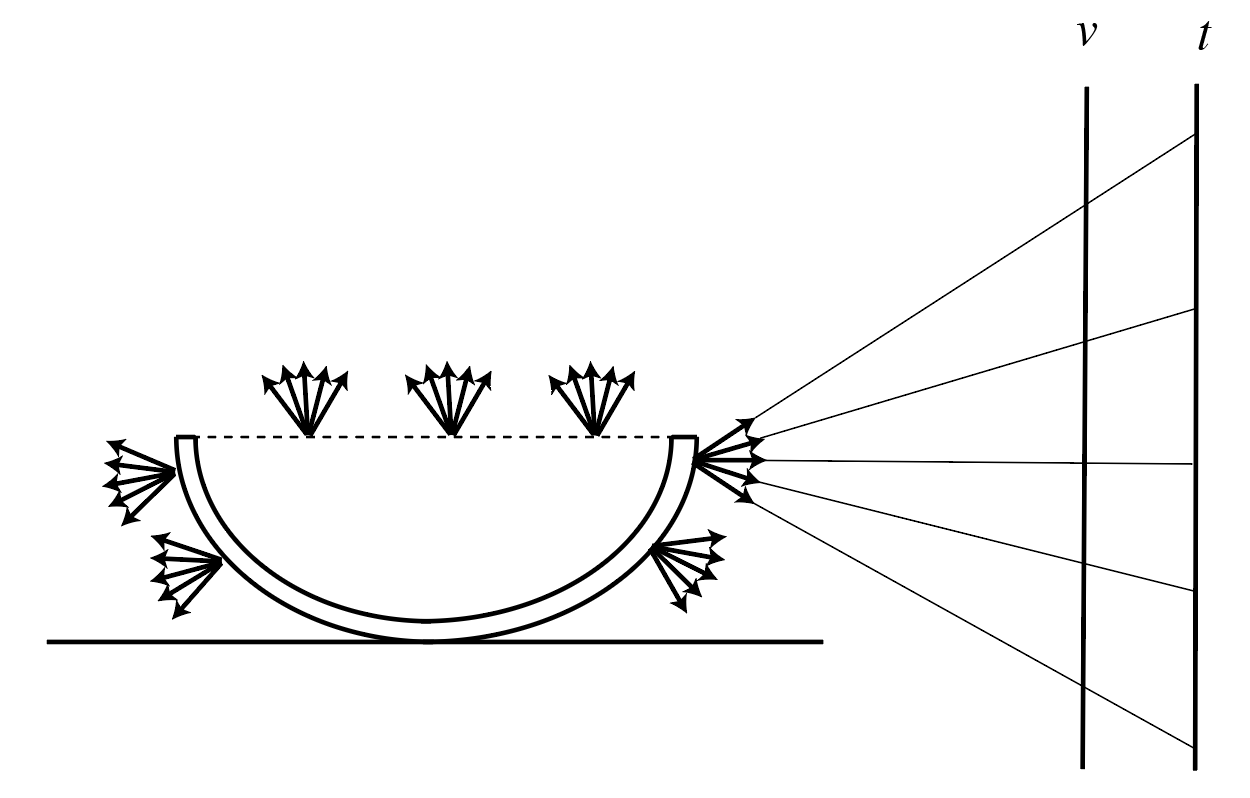
\includegraphics[width=2.5in]{images/convexhull.png}
    
    \caption{Two plane parameterisation (left): the plenoptic function can be described by the radiance along a ray passing through two parallel planes. The free space assumption (right): if we consider only the bundle of rays leaving from the convex hull of the object at a particular instance in time, in a single colour channel, we can parameterise the light rays as a function of 4 variables rather than 7.}
    
    \label{convexhull}
\end{figure}

Also illustrated is a common convention for describing light rays in this 4 dimensional space called the two plane parameterisation. In this parameterisation, two parallel planes are used to fix both the position and orientation of each ray by fixing their points of intersection with two parallel planes. By convention, the plane closest to the scene it termed \textit{u, v} and the plane closest to the camera sensor is the \textit{s, t} plane.


This 4D realisation of the light field originated as a model of rendering 3D computer graphics, one which shifted emphasis from notions of texture and geometric primitives to modelling the behaviour of light rays permeating space. Since then however, the conceptual framework of the light field has drawn a following of researchers at an intersecting region of signal processing, computer vision and robotics \cite{dansereau2014phd}. This notion of light field imaging finds a foothold in this thesis project through the utilisation of camera arrays, which are devices that sample multiple views of the same scene. Using a camera array is a simple method for acquiring a dense sample of the light field, where the position of the camera determines \textit{(s,t)} while the location of the pixel determines \textit{(u, v)} \cite{yao2016camarray}. The images captured from a camera array are mapped easily to the 4D light field, and identifying corresponding pixels across images exposes a rich tapestry of geometric information about the scene. 

\begin{figure}[htbp]
    \centering
    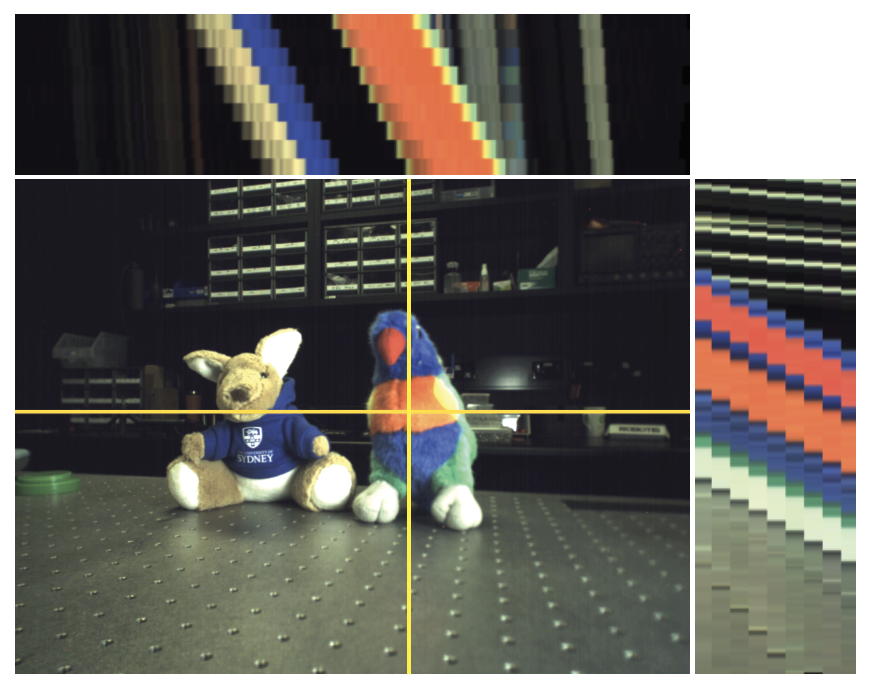
\includegraphics[width=1.6in]{images/epipolarimage.png}
    
\includegraphics[width=0.4in]{images/blank.png}
    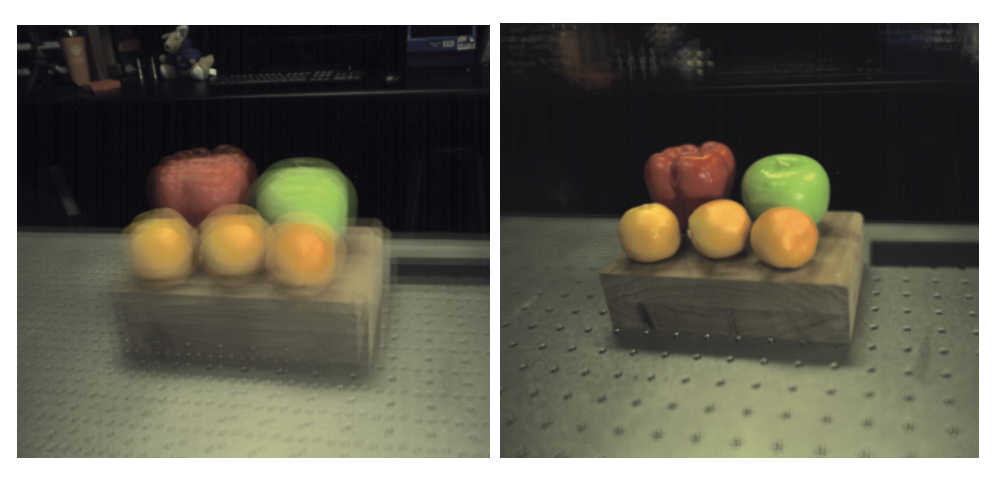
\includegraphics[width=3.5in]{images/fruitfocus.png}
    \caption{Epipolar Plane Images (left): Shown as a slice of a volume, the images formed by dissecting the image in the \textit{s,u} and \textit{t,v} planes are characterised by sheared straight lines, with the grade of the slope encoding the amount of parallax experienced by a pixel at that \textit{u} or \textit{v} coordinate. Synthetic aperture focusing (right): taking the average of every image from the camera array yields an image where different parts are in focus depending on the alignments of the images.}
    \label{epiplaneimg}
\end{figure}


One way that this geometric information can be easily visualised is by taking slices of the light field image in the \textit{s,u} or \textit{t, v} axes as shown in figure \ref{epiplaneimg}. While the idea of taking a 2D slice from the 4D image can seem complex, the task of generating a so called 'epipolar plane image' from a camera array is deceptively simple. Images captured from camera arrays can be stacked to form a solid volume, from which 2D slices can be sampled. Each of these slices yields an image characterised by sheared straight lines, encoding information about the geometry of the scene, including depth and occlusions \cite{bolles1987epiplane}. 

The geometric information encoded in a light field sampling can alternatively be visualised by processing the image into a 'focal stack'. Focal stacks closely resemble images with shallow depth of field such as those that can be captured from a commercial camera. Light field focal stacks differ from focus in the optical sense however in that they are synthetic and can be recomputed after the image has been taken, effectively allowing control over the depth of field and focal depth in post-processing. Focal stacks can be computed from camera array images by layering images over one another and taking the average value for each pixel. The result is that parts of the scene that closely overlap appear in focus while areas with poor overlap create a 'bokeh' effect. More formally, if the relative pose of each camera is known, a specific focal stack for any desired depth can be computed by projecting each image onto the desired focal plane, and computing their average \cite{vaish2004parallax}.

These representations of the light field will play an important role in this thesis project as we experiment with different methods for feeding light field images to the machine learning pipeline. An important consideration in any machine learning algorithm is the feature space - based on what particular inputs will the algorithm be making its decision? Raw images contain millions of measurements and thus represent an incredibly high-dimensional feature space for neural networks to process. Light field images are several times larger, and thus it is important that some form of dimensionality reduction is used to ease the training process. With the goal of investigating effective methods of feeding light fields to neural networks, this thesis will explore the use of three different light field formats as the entry point to the machine learning pipeline. The first two will be the focal stack, and epipolar plane image described above, interpreting the images as a 3 dimensional volume created by stacking 2 dimensional images on top of one another. The third will treat the light field as a 4 dimensional volume, requiring a 3D signal processing pipeline to fully take advantage of the dimensionality.


\section{Machine Learning for Image Processing}



\section{Depth Estimation and Visual Odometry}

Since the very beginning of photography, cameras have captured 2D representations of a 3D world, meaning information about physical structure is lost. With the addition of a second viewpoint however we can learn a little more about the shape of the scene as governed by epipolar geometry \cite{zisserman2004multiview}. Meanwhile, a video is a sequence of images, taken in very quick succession, and so one could think of video footage as a multi-view camera where each image is separated not only spatially but also temporally. Identifying the amount of motion between two temporal frames of a single camera is the goal of visual odometry, but it is also problematic because with a single camera there is no way of concretely discerning the actual magnitude of the movement based on pixel data alone, requiring a scale factor estimate based on features in the image \cite{gakne2018scale, nister2004vo, zhou2016scale, zhou2019scale}. In fact, this scale ambiguity is often exploited by film makers - what appears as a sweeping shot of a vast landscape on the big screen is often modeled as a miniature film set in the studio. Because the image is monocular, there is no way to ground our measurements of scale in real world units, and so we resort to our imaginations to fill in the gaps. What \textit{is} preserved in these monocular setups however is the overall structure of the scene and motion of the camera - we may not know how large the object is or how far the camera has moved, but we \textit{can} compute the shape of the object as well as the direction of camera motion.


The two core objectives of this thesis are related intimately by the geometric constraints that are present in such multi-view imaging setups - in order to infer something about how a camera has moved from one image to another, one would first need to know something about the shape of the scene being imaged. The problem of discerning scene geometry from a sequence of spatially adjusted images is referred to as 'structure from motion' (SfM). Likewise, given knowledge of how the camera has moved from one frame to another, 3D coordinates for each set of corresponding points in those images can be triangulated. Estimating both simultaneously is the subject of this thesis, and is a useful outcome for applications such as autonomous robotics navigating unknown environments, and Simultaneous Localisation and Mapping (SLAM).


An intuitive idea is to identify the direction of movement of each pixel between the two images, however one would find that unless every point in the scene lies on a single plane, each pixel moves a different amount according to its distance to the camera. Governed by parallax, not only does the relative motion of each pixel depend on the corresponding light ray's location of origin, but the colour and intensity of those pixels may change drastically if the scene contains shiny objects.

One recent approach that has driven a large body of research is a machine learning based pipeline that relies on two 

\chapter{Progress Report}

\chapter{Updated Research Proposal}


\newpage

%\newpage
\bibliographystyle{plain}
\bibliography{bibliography.bib}

\end{document}
